\section{Kết quả thực nghiệm}
\subsection{Dữ liệu thực nghiệm}
% Randomized data
\subsubsection{Randomized data}
\begin{table}[!h]
    \centering
    \caption{Sorting Algorithms Performance (Data size: 10,000 to 50,000)}
    \resizebox{\textwidth}{!}{
    \begin{tabular}{|c|c|c|c|c|c|c|}
    \hline
    \multicolumn{7}{|c|}{Data order: Randomize} \\ \hline
    \textbf{Data size}         & \multicolumn{2}{c|}{10,000} & \multicolumn{2}{c|}{30,000} & \multicolumn{2}{c|}{50,000} \\ \hline
    \textbf{Resulting statics} & Running time    & Comparisons & Running time & Comparisons & Running time   & Comparisons   \\ \hline
    Selection sort             & $32.183573$     & $100009999$ & $306.653455$ & $900029999$ & $844.855146$   & $2500049999$  \\ \hline
    Insertion sort             & $19.384731$     & $50522006$  & $145.740501$ & $452272024$ & $392.687566$   & $1248436921$  \\ \hline
    Bubble sort                & $70.734463$     & $100009999$ & $934.530289$ & $900029999$ & $3299.414892$  & $2500049999$  \\ \hline
    Shaker sort                & $42.287156$     & $66875081$  & $619.416315$ & $600759308$ & $2055.377927$  & $1665041683$  \\ \hline
    Shell sort                 & $0.986861$      & $652068$    & $4.293509$   & $2270237$   & $10.13297$     & $4405508$     \\ \hline
    Heap sort                  & $0.960662$      & $637548$    & $3.341052$   & $2150596$   & $5.735989$     & $3772079$     \\ \hline
    Merge sort                 & $1.149464$      & $588901$    & $6.414518$   & $1955125$   & $9.465082$     & $3410940$     \\ \hline
    Quick sort                 & $0.665371$      & $284724$    & $2.19808$    & $943182$    & $3.667631$     & $1652882$     \\ \hline
    Counting sort              & $0.097903$      & $50000$     & $0.288228$   & $150000$    & $0.567188$     & $250001$      \\ \hline
    Radix sort                 & $0.282387$      & $130057$    & $1.10427$    & $480071$    & $1.811559$     & $800071$      \\ \hline
    Flash sort                 & $0.360212$      & $124341$    & $1.604112$   & $344133$    & $2.174185$     & $581725$      \\ \hline
    \end{tabular}}
    \end{table}

\begin{table}[!h]
    \centering
    \caption{Sorting Algorithms Performance (Data size: 100,000 to 500,000)}
    \resizebox{\textwidth}{!}{
    \begin{tabular}{|c|c|c|c|c|c|c|}
    \hline
    \multicolumn{7}{|c|}{Data order: Randomize} \\ \hline
    \textbf{Data size}         & \multicolumn{2}{c|}{100,000} & \multicolumn{2}{c|}{300,000} & \multicolumn{2}{c|}{500,000}   \\ \hline
    \textbf{Resulting statics} & Running time    & Comparisons   & Running time   & Comparisons   & Running time  & Comparisons     \\ \hline
    Selection sort             & $3349.233902$   & $10000099999$ & $31423.71571$  & $90000299999$ & $85183.64454$ & $250000499999$  \\ \hline
    Insertion sort             & $1724.785371$   & $4991334689$  & $15283.73471$  & $45004491273$ & $42641.65251$ & $125061559509$  \\ \hline
    Bubble sort                & $13368.79662$   & $10000099999$ & $122968.1562$  & $90000299999$ & $342455.073$  & $250000499999$  \\ \hline
    Shaker sort                & $8192.499752$   & $6630746484$  & $74832.3415$   & $60042574753$ & $207449.4541$ & $16651086366$   \\ \hline
    Shell sort                 & $12.283542$     & $1021936$     & $41.400131$    & $36211086$    & $80.487939$   & $66162103$      \\ \hline
    Heap sort                  & $12.267843$     & $8044268$     & $50.151986$    & $26488066$    & $74.984454$   & $45966994$      \\ \hline
    Merge sort                 & $19.772601$     & $7221288$     & $43.158881$    & $23550740$    & $73.601204$   & $40684963$      \\ \hline
    Quick sort                 & $7.561674$      & $3537485$     & $29.876757$    & $11648573$    & $41.883683$   & $19765518$      \\ \hline
    Counting sort              & $1.102757$      & $500001$      & $3.475312$     & $1500001$     & $6.097413$    & $2500001$       \\ \hline
    Radix sort                 & $3.627125$      & $1600071$     & $12.835631$    & $5700085$     & $27.51946$    & $9000085$       \\ \hline
    Flash sort                 & $5.305346$      & $1179306$     & $18.403426$    & $3560788$     & $32.058046$   & $5776314$       \\ \hline
    \end{tabular}}
    \end{table}

    \begin{figure}[H]
        \centering
        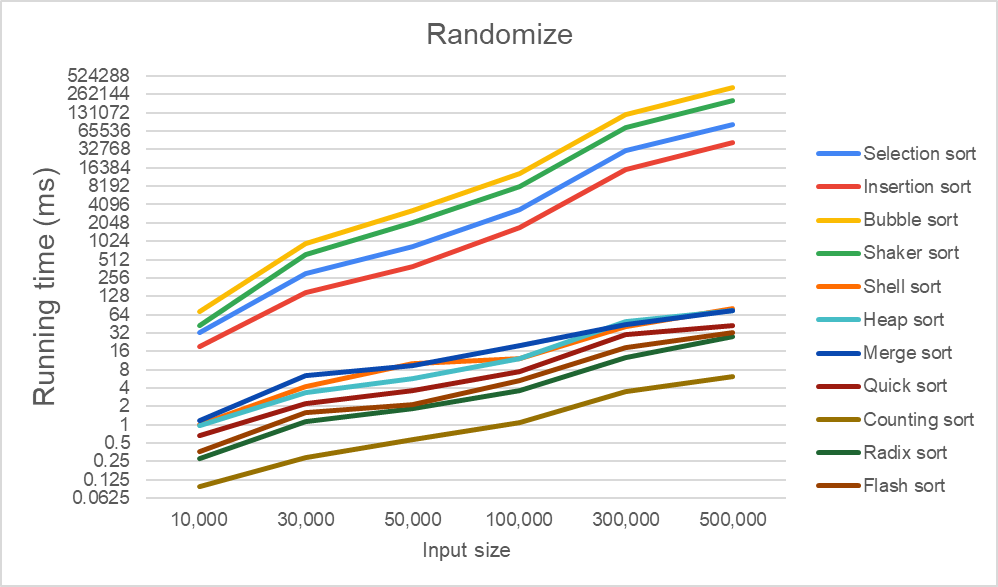
\includegraphics[width = 0.9\linewidth]{img/experiment/running time/randomized/1.png}
        \caption{Thời gian chạy của các thuật toán sắp xếp với dữ liệu ngẫu nhiên}
    \end{figure}

    \begin{figure}[H]
        \centering   
        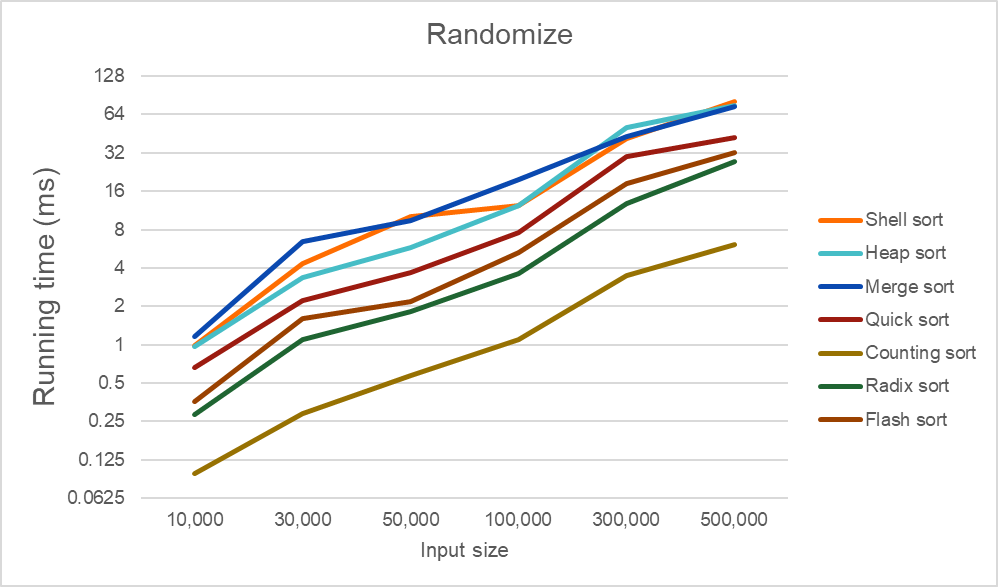
\includegraphics[width = 0.9\linewidth]{img/experiment/running time/randomized/2.png}
        \caption{Thời gian chạy của các thuật toán chạy nhanh sắp xếp với dữ liệu ngẫu nhiên}
    \end{figure}

    \begin{figure}[H]
        \centering        
        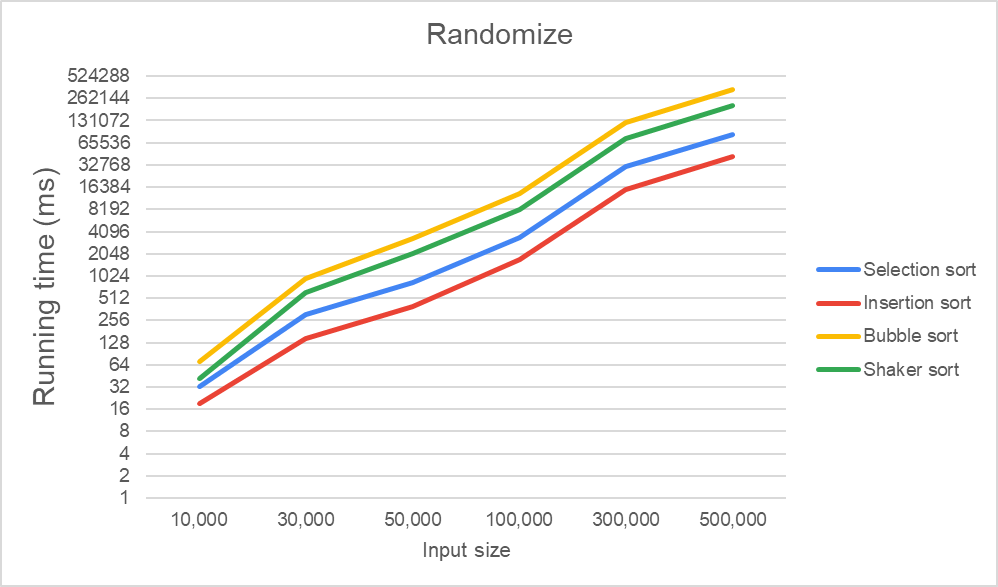
\includegraphics[width = 0.9\linewidth]{img/experiment/running time/randomized/3.png}
        \caption{Thời gian chạy của các thuật toán chạy chậm sắp xếp với dữ liệu ngẫu nhiên}
    \end{figure}

    \paragraph{Quan sát biểu đồ đường:}
    \begin{itemize}
        \item \textbf{Hiệu năng tốt nhất:} Counting sort.
        \item \textbf{Hiệu năng tệ nhất:} Bubble sort.
        \item \textit{Selection sort, Insertion sort, Bubble sort, Shaker sort :} Các thuật toán này đều có thời gian tăng nhanh theo kích thước của bộ dữ liệu, điều này phù hợp với độ phức tạp lý thuyết $\mathcal{O}(n^2)$ của chúng.
        \item \textit{Shell sort:} Mặc dù về lý thuyết \textit{Shell sort} có độ phức tạp trung bình là $\mathcal{O}(n^{3/2})$ nhưng kết quả thực nghiệm lại thể hiện rằng nó có thời gian chạy nằm chung nhóm với các thuật toán có độ phức tạp $\mathcal{O}(n \cdot \log n)$. 
        \item \textit{Heap sort, Merge sort, Quick sort:} Các thuật toán đều có thời gian chạy ổn định và tăng chậm, phù hợp với độ phức tạp $\mathcal{O}(n \cdot \log n)$.
        \item \textit{Counting sort, Radix sort, Flash sort:} Các thuật toán này sử dụng phương pháp phân phối dữ liệu nên với bất kì bộ dữ liệu ngẫu nhiên nào thời gian chạy của chúng cũng tương đối ổn định. Giúp duy trì hiệu năng tốt kể cả khi kích thước của bộ dữ liệu tăng lên.
    \end{itemize}

    \newpage
    \begin{figure}[H]
        \centering        
        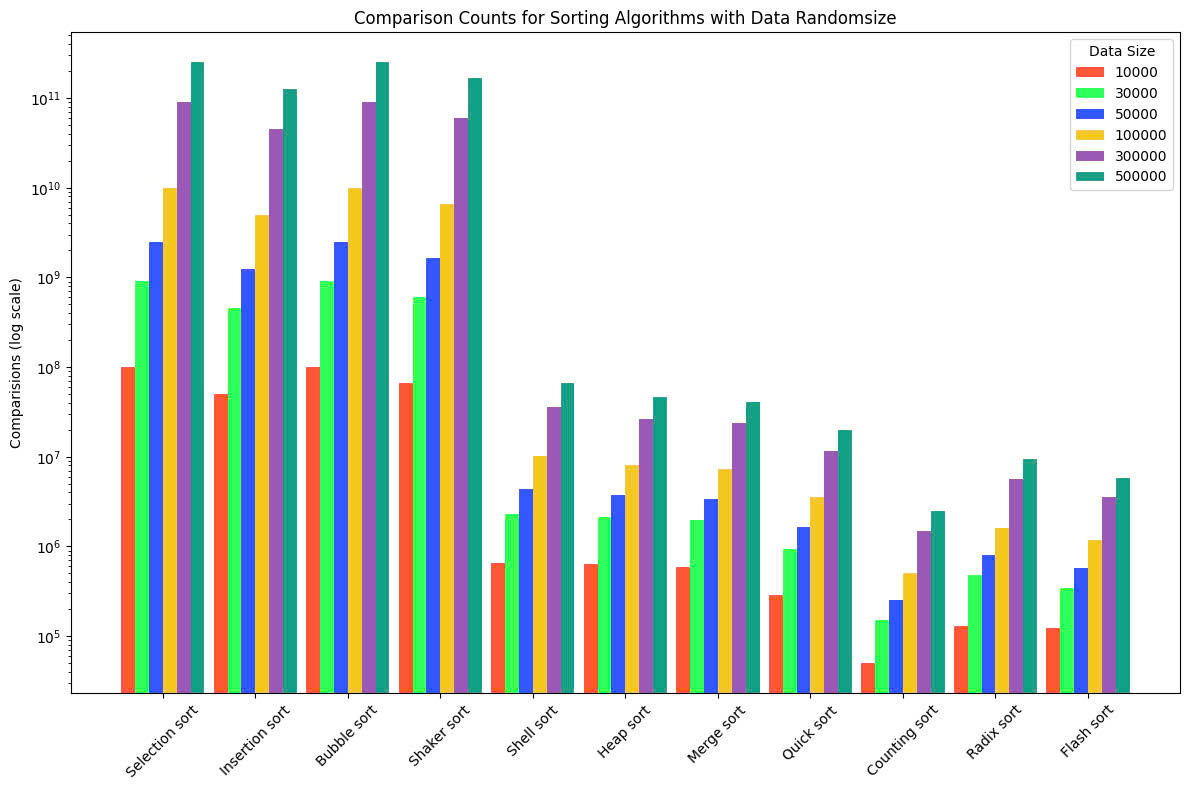
\includegraphics[width = 1\linewidth]{img/experiment/comparison/comparision_randomesize.jpg}
        \caption{Biểu đồ số lượng phép so sánh của các thuật toán trên bộ dữ liệu ngẫu nhiên}
    \end{figure}
    \paragraph{Quan sát biểu đồ cột:}
    \begin{itemize}
        \item \textbf{Số phép so sánh ít nhất:} Counting sort.
        \item \textbf{Số phép so sánh nhiều nhất:} Selection sort.
        \item \textit{Selection sort, Bubble sort, Insert sort, Shaker sort:} Các thuật toán này đều có số phép so sánh nhiều nhất và số phép tang nhanh khi kích thước mảnh tăng lên. \textit{Selection sort} là thuật toán có nhiều phép so sánh nhất trong nhóm này vì luôn phải thực hiện n(n-1)/2 phép so sánh mà không phụ thuộc vào tính chất bộ dữ liệu.
        \item \textit{Shell sort, Heap sort, Merge sort, Quick sort:} Các thuật toán này đều có số phép so sánh ít nhất và tăng chậm khi kích thước mảng tăng lên. \textit{Quick sort} vẫn là thuật toán có hiệu năng tốt nhất trong nhóm này  khi xử lý dữ liệu ngẫu nhiên nhờ chiến lược chia để trị. Số phép so sánh tăng chậm khi kích thước mảng tăng, làm cho thuật toán này trở thành một trong những lựa chọn tốt nhất trong các trường hợp tổng quát.
        \item \textit{Counting sort, Radix sort, Flash sort:} Các thuật toán này sắp xếp đều không phụ thuộc vào việc so sánh giữa giá trị của các phần tử nên có số phép so sánh ít nhất và không tăng nhanh khi kích thước mảng tăng lên.
    \end{itemize}
\newpage
%-------------------------------------------------------------------------------------------
% Sorted data
\subsubsection{Sorted data}
\begin{table}[!h]
    \centering
    \caption{Sorting Algorithms Performance (Data size: 10,000 to 50,000)}
    \resizebox{\textwidth}{!}{
    \begin{tabular}{|c|c|c|c|c|c|c|}
    \hline
    \multicolumn{7}{|c|}{Data order: Sorted} \\ \hline
    \textbf{Data size}         & \multicolumn{2}{c|}{10,000} & \multicolumn{2}{c|}{30,000} & \multicolumn{2}{c|}{50,000} \\ \hline
    \textbf{Resulting statics} & Running time    & Comparisons & Running time & Comparisons & Running time   & Comparisons   \\ \hline
    Selection sort             & $32.454305$     & $100009999$ & $327.066795$ & $900029999$ & $811.842781$   & $2500049999$  \\ \hline
    Insertion sort             & $0.03214$       & $29998$     & $0.094828$   & $89998$     & $0.149148$     & $149998$      \\ \hline
    Bubble sort                & $63.250497$     & $100009999$ & $452.859471$ & $900029999$ & $1207.410159$  & $2500049999$  \\ \hline
    Shaker sort                & $0.023744$      & $20002$     & $0.065392$   & $60002$     & $0.109364$     & $100002$      \\ \hline
    Shell sort                 & $0.233536$      & $360042$    & $0.717699$   & $1170050$   & $1.269428$     & $2100049$     \\ \hline
    Heap sort                  & $0.731515$      & $670329$    & $2.266307$   & $2236648$   & $3.914161$     & $3925351$     \\ \hline
    Merge sort                 & $0.605551$      & $539850$    & $1.867132$   & $1779418$   & $3.338597$     & $3105338$     \\ \hline
    Quick sort                 & $0.156341$      & $193611$    & $0.475848$   & $627227$    & $0.769475$     & $1084459$     \\ \hline
    Counting sort              & $0.0907$        & $50001$     & $0.272008$   & $150001$    & $0.542011$     & $250001$      \\ \hline
    Radix sort                 & $0.496967$      & $130057$    & $1.313971$   & $480071$    & $2.314367$     & $800071$      \\ \hline
    Flash sort                 & $0.409824$      & $157987$    & $0.813127$   & $473987$    & $1.384683$     & $789987$      \\ \hline
    \end{tabular}}
\end{table}

\begin{table}[!h]
    \centering
    \caption{Sorting Algorithms Performance (Data size: 100,000 to 500,000)}
    \resizebox{\textwidth}{!}{
    \begin{tabular}{|c|c|c|c|c|c|c|}
    \hline
    \multicolumn{7}{|c|}{Data order: Sorted} \\ \hline
    \textbf{Data size}         & \multicolumn{2}{c|}{100,000} & \multicolumn{2}{c|}{300,000} & \multicolumn{2}{c|}{500,000}   \\ \hline
    \textbf{Resulting statics} & Running time    & Comparisons   & Running time   & Comparisons   & Running time  & Comparisons     \\ \hline
    Selection sort             & $3420.596541$   & $10000099999$ & $30403.08904$  & $90000299999$ & $84546.66351$ & $250000499999$  \\ \hline
    Insertion sort             & $0.293327$      & $299998$      & $0.878459$     & $899998$      & $1.55454$     & $1499998$       \\ \hline
    Bubble sort                & $4995.281004$   & $10000099999$ & $44724.22977$  & $90000299999$ & $123768.8695$ & $250000499999$  \\ \hline
    Shaker sort                & $0.207387$      & $200002$      & $0.640425$     & $600002$      & $1.112155$    & $1000002$       \\ \hline
    Shell sort                 & $2.711568$      & $4500051$     & $9.147943$     & $15300061$    & $14.070404$   & $25500058$      \\ \hline
    Heap sort                  & $8.039268$      & $8365080$     & $25.626199$    & $27413230$    & $44.345756$   & $47404886$      \\ \hline
    Merge sort                 & $6.695373$      & $6560682$     & $25.754188$    & $21324394$    & $36.377894$   & $36710346$      \\ \hline
    Quick sort                 & $1.556683$      & $2268923$     & $5.091156$     & $7275707$     & $8.709876$    & $12475707$      \\ \hline
    Counting sort              & $1.117524$      & $500001$      & $3.133094$     & $1500001$     & $5.192094$    & $2500001$       \\ \hline
    Radix sort                 & $4.611011$      & $1600071$     & $16.120228$    & $5700085$     & $27.212628$   & $9500085$       \\ \hline
    Flash sort                 & $2.819439$      & $1579987$     & $8.235912$     & $4739987$     & $14.235853$   & $7899987$       \\ \hline
    \end{tabular}}
\end{table}

\begin{figure}[H]
    \centering   
    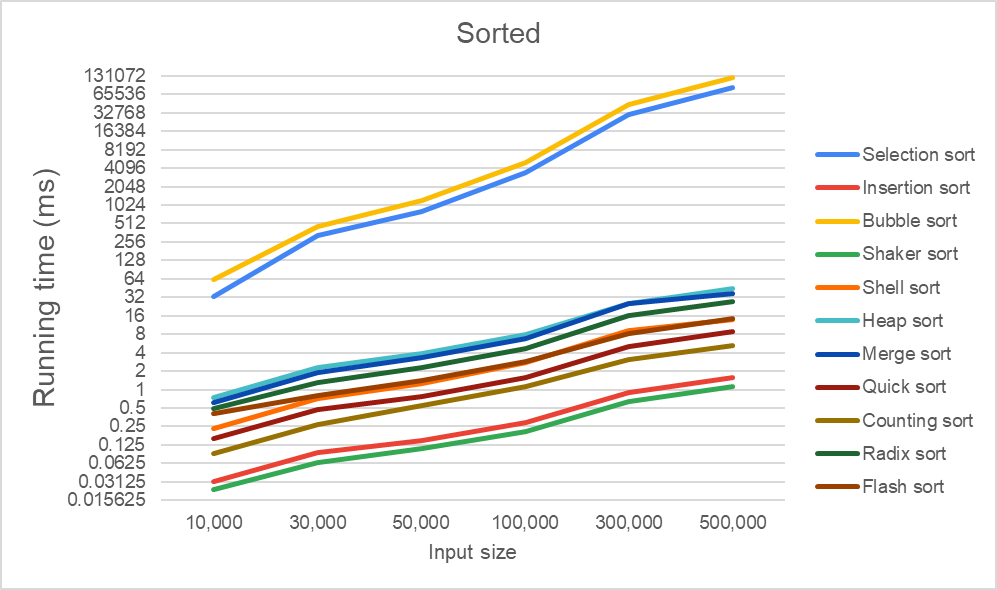
\includegraphics[width = 0.9\linewidth]{img/experiment/running time/sorted/1.png}
    \caption{Thời gian chạy của các thuật toán sắp xếp với dữ liệu đã sắp xếp}
\end{figure}

\begin{figure}[H]
    \centering   
    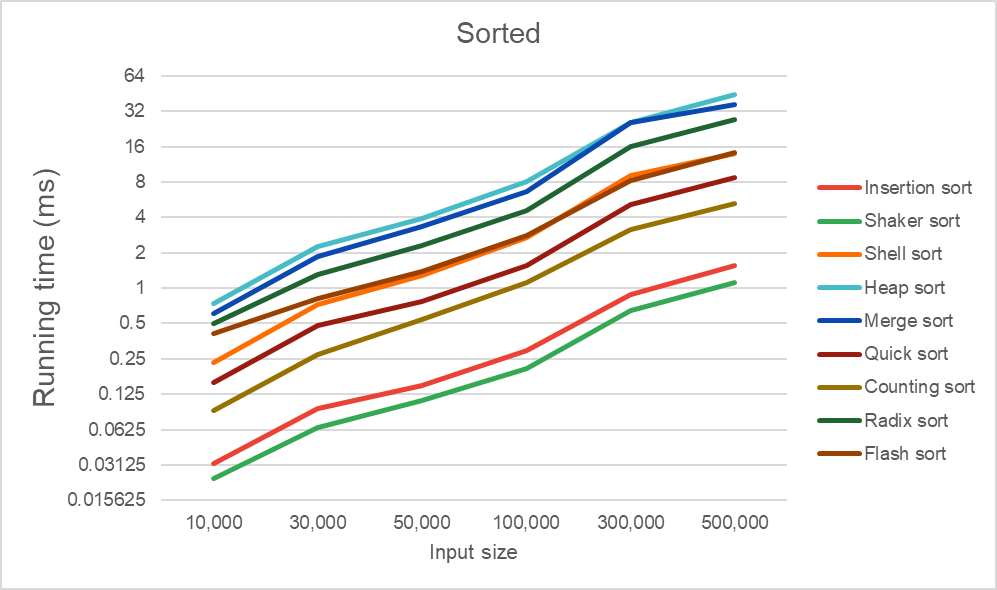
\includegraphics[width = 0.9\linewidth]{img/experiment/running time/sorted/2.png}
    \caption{Thời gian chạy của các thuật toán chạy nhanh sắp xếp với dữ liệu đã sắp xếp}     
\end{figure}

\begin{figure}[H]
    \centering   
    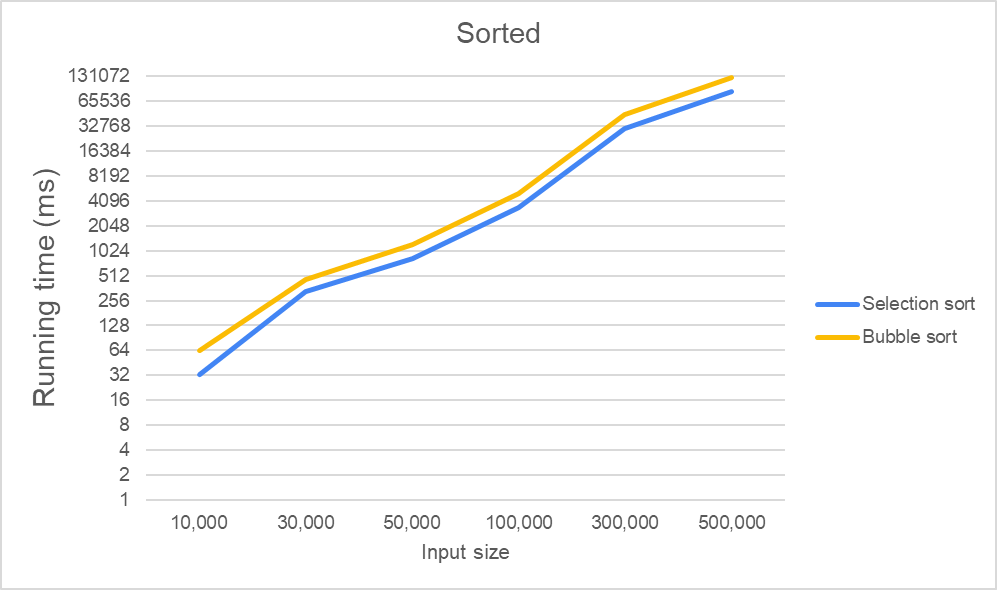
\includegraphics[width = 0.9\linewidth]{img/experiment/running time/sorted/3.png}
    \caption{Thời gian chạy của các thuật toán chạy chậm sắp xếp với dữ liệu đã sắp xếp}
\end{figure}

    \paragraph{Quan sát biểu đồ đường:}
    \begin{itemize}
        \item \textbf{Hiệu năng tốt nhất:} Shaker sort.
        \item \textbf{Hiệu năng tệ nhất:} Bubble sort.
        \item Vì bộ dữ liệu đã được sắp xếp nên sẽ có một số thuật toán ít phải thực hiện phép so sánh, hoán đổi vị trí và một số sẽ nhận diện được bộ dữ liệu đã được sắp xếp, giúp cải thiện đáng kể thời gian chạy.
        \item \textit{Selection sort, Bubble sort: } Kể cả bộ dữ liệu đã được sắp xếp nhưng vì tính chất thuật toán này vẫn phải thực hiện số lượng phép so sánh và hoán đổi vị trí, do đó thời gian chạy của chúng vẫn tăng nhanh theo kích thước của bộ dữ liệu.
        \item \textit{Insertion sort, Shaker sort: } Hai thuật toán này có thể nhận diện được bộ dữ liệu đã được sắp xếp nên thời gian chạy của chúng giảm đáng kể, nằm trong nhóm có hiệu năng tốt nhất. Vì chúng chỉ cần duyệt qua mảng một lần và không cần phải hoán đổi vị trí, 
        \item \textit{Shell sort: } Tuy là một biến thể của \textit{Insertion sort} nhưng \textit{Shell sort} lại không thể nhận diện được bộ dữ liệu đã được sắp xếp nên không giảm được thời gian chạy. Tuy vậy thời gian chạy của nó vẫn ổn định và không tăng nhanh khi kích thước mảng tăng.
        \item \textit{Heap sort, Merge sort, Quick sort: } Các thuật toán này đều có thời gian chạy ổn định và tăng chậm, phù hợp với độ phức tạp $\mathcal{O}(n \cdot \log n)$. \textit{Quick sort} với phương pháp chọn pivot nằm giữa mảng đã giúp tránh được các tình huống xấu nhất khi gọi đệ quy, bảo đảm việc chia nhóm đều hơn, giúp giảm thời gian chạy so với \textit{Heap sort} và \textit{Merge sort}.
        \item \textit{Counting sort, Radix sort, Flash sort: } Các thuật toán này sử dụng phương pháp phân phối dữ liệu nên với bộ dữ liệu được sắp xếp thì các thuật toán này sẽ chia mảng ra đều hơn, giúp hiệu năng của chúng được duy trì tốt.
    \end{itemize}    

    \newpage
    \begin{figure}[H]
        \centering
        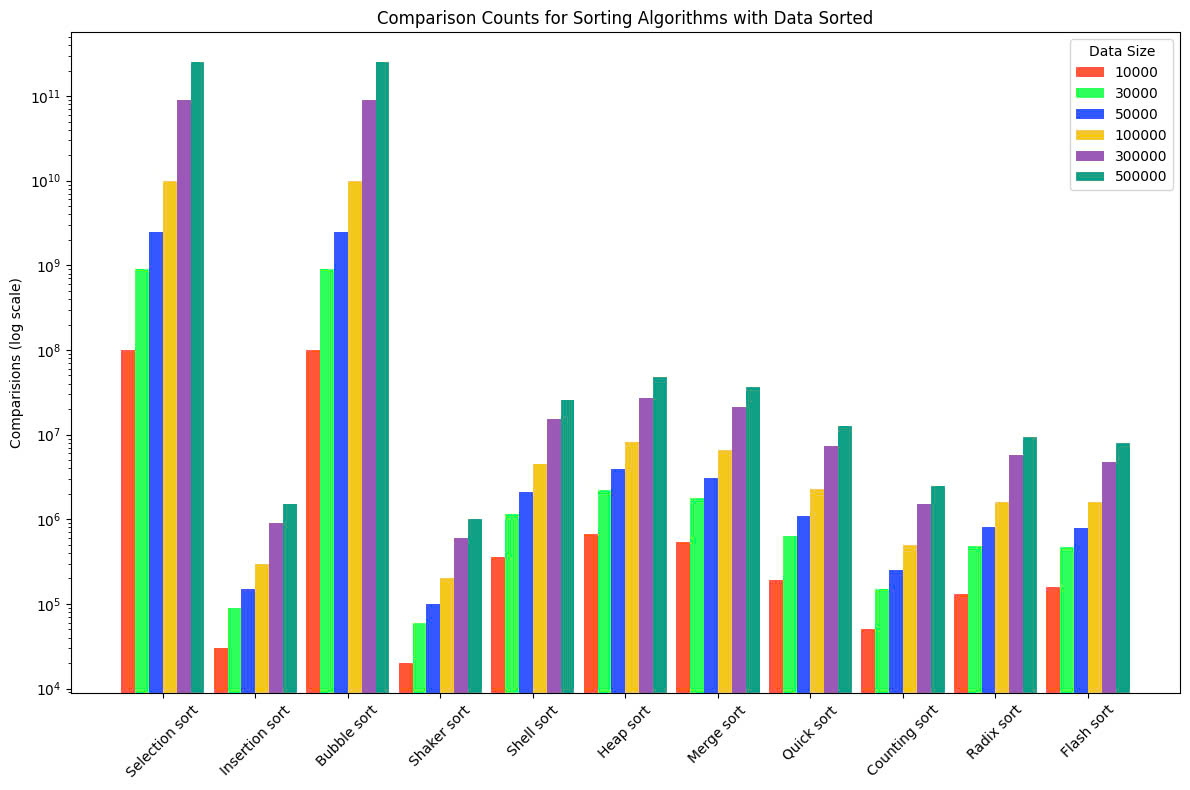
\includegraphics[width = 1\linewidth]{img/experiment/comparison/COMPARISON_SORTED.jpg}
        \caption{Biểu đồ số lượng phép so sánh của các thuật toán trên bộ dữ liệu đã sắp xếp}
    \end{figure}
    \paragraph{Quan sát biểu đồ cột:}
    \begin{itemize}
        \item \textbf{Số phép so sánh ít nhất:} Insertion sort.
        \item \textbf{Số phép so sánh nhiều nhất:} Selection sort.
        \item \textit{Selection sort, Bubble sort:} Các thuật toán này đều có số phép so sánh nhiều nhất và số phép tang nhanh khi kích thước mảnh tăng lên. \textit{Selection sort} là thuật toán có nhiều phép so sánh nhất trong nhóm này vì luôn phải thực hiện n(n-1)/2 phép so sánh mà không phụ thuộc vào tính chất bộ dữ liệu. 
        \item \textit{Insertion sort, Shaker sort: }Khi dữ liệu đã được sắp xếp, \textit{Insertion sort} và \textit{Shaker sort} chỉ thực hiện một số lượng nhỏ phép so sánh vì thuật toán nhận ra dữ liệu đã có thứ tự sau một lần duyệt. Số phép so sánh tăng chậm khi kích thước mảng tăng.
        \item \textit{Merge sort, Shell sort, Heap sort, Quick sort: }Số phép so sánh ổn định bất kể dữ liệu đã được sắp xếp. Đặc biệt đối với \textit{Quick sort} với chiến lược chọn pivot ở giữa giúp giảm số phép so sánh so với các thuật toán khác.
        \item \textit{Counting sort, Radix sort, Flash sort:} Các thuật toán này sắp xếp đều không phụ thuộc vào việc so sánh giữa giá trị của các phần tử nên có số phép so sánh ít nhất và không tăng nhanh khi kích thước mảng tăng lên vì nó không dựa vào việc so sánh phần tử.
    \end{itemize}

\newpage

%-------------------------------------------------------------------------------------------
% Nearly sorted data
\subsubsection{Nearly sorted data}
\begin{table}[!h]
    \centering
    \caption{Sorting Algorithms Performance (Data size: 10,000 to 50,000)}
    \resizebox{\textwidth}{!}{
    \begin{tabular}{|c|c|c|c|c|c|c|}
    \hline
    \multicolumn{7}{|c|}{Data order: Nearly sorted} \\ \hline
    \textbf{Data size}         & \multicolumn{2}{c|}{10,000} & \multicolumn{2}{c|}{30,000} & \multicolumn{2}{c|}{50,000} \\ \hline
    \textbf{Resulting statics} & Running time    & Comparisons & Running time & Comparisons & Running time   & Comparisons   \\ \hline
    Selection sort             & $33.777678$     & $100009999$ & $300.012069$ & $900029999$ & $1099.69264$   & $2500049999$  \\ \hline
    Insertion sort             & $0.149949$      & $168826$    & $0.208278$   & $372634$    & $0.388123$     & $641438$      \\ \hline
    Bubble sort                & $71.653936$     & $100009999$ & $464.134654$ & $900029999$ & $2001.063413$  & $2500049999$  \\ \hline
    Shaker sort                & $0.103333$      & $126542$    & $0.27345$    & $495592$    & $1.438943$     & $984696$      \\ \hline
    Shell sort                 & $0.284$         & $400830$    & $1.561852$   & $1317798$   & $2.344271$     & $2419280$     \\ \hline
    Heap sort                  & $0.719923$      & $669816$    & $3.287426$   & $2236506$   & $3.859756$     & $3925382$     \\ \hline
    Merge sort                 & $0.664989$      & $552976$    & $2.02201$    & $1820034$   & $3.262733$     & $3183125$     \\ \hline
    Quick sort                 & $0.170889$      & $193651$    & $0.49362$    & $627271$    & $1.165753$     & $1084499$     \\ \hline
    Counting sort              & $0.098644$      & $50001$     & $0.256398$   & $150001$    & $0.566396$     & $250001$      \\ \hline
    Radix sort                 & $0.25174$       & $130057$    & $1.27655$    & $480071$    & $1.639467$     & $800071$      \\ \hline
    Flash sort                 & $0.209551$      & $157949$    & $0.650804$   & $473955$    & $1.294377$     & $789943$      \\ \hline
    \end{tabular}}
    \end{table}

\begin{table}[!h]
\centering
\caption{Sorting Algorithms Performance (Data size: 100,000 to 500,000)}
\resizebox{\textwidth}{!}{
\begin{tabular}{|c|c|c|c|c|c|c|}
\hline
\multicolumn{7}{|c|}{Data order: Nearly sorted} \\ \hline
\textbf{Data size}         & \multicolumn{2}{c|}{100,000} & \multicolumn{2}{c|}{300,000} & \multicolumn{2}{c|}{500,000}   \\ \hline
\textbf{Resulting statics} & Running time    & Comparisons   & Running time   & Comparisons   & Running time  & Comparisons     \\ \hline
Selection sort             & $3371.550636$   & $10000099999$ & $30445.65322$  & $90000299999$ & $89733.04115$ & $250000499999$  \\ \hline
Insertion sort             & $0.739959$      & $1543470$     & $3.404998$     & $5556766$     & $5.04694$     & $7276634$       \\ \hline
Bubble sort                & $7233.954453$   & $10000099999$ & $44954.00437$  & $90000299999$ & $125495.1535$ & $250000499999$  \\ \hline
Shaker sort                & $1.631161$      & $1711197$     & $3.407664$     & $5263822$     & $5.415176$    & $8201076$       \\ \hline
Shell sort                 & $3.551392$      & $5020837$     & $10.427654$    & $16637181$    & $18.093586$   & $27866736$      \\ \hline
Heap sort                  & $9.545368$      & $8363632$     & $25.528625$    & $27416975$    & $67.038805$   & $47416196$      \\ \hline
Merge sort                 & $9.915788$      & $6727044$     & $24.500308$    & $21849463$    & $47.313286$   & $37366559$      \\ \hline
Quick sort                 & $2.503859$      & $2268963$     & $7.891514$     & $7275747$     & $13.975123$   & $12475747$      \\ \hline
Counting sort              & $1.137761$      & $500001$      & $3.095672$     & $1500001$     & $5.480158$    & $2500001$       \\ \hline
Radix sort                 & $3.494295$      & $1600071$     & $12.653055$    & $5700085$     & $21.684501$   & $9500085$       \\ \hline
Flash sort                 & $2.815089$      & $1579943$     & $12.262283$    & $4739952$     & $14.734613$   & $7899958$       \\ \hline
\end{tabular}}
\end{table}

\begin{figure}[H]
    \centering
    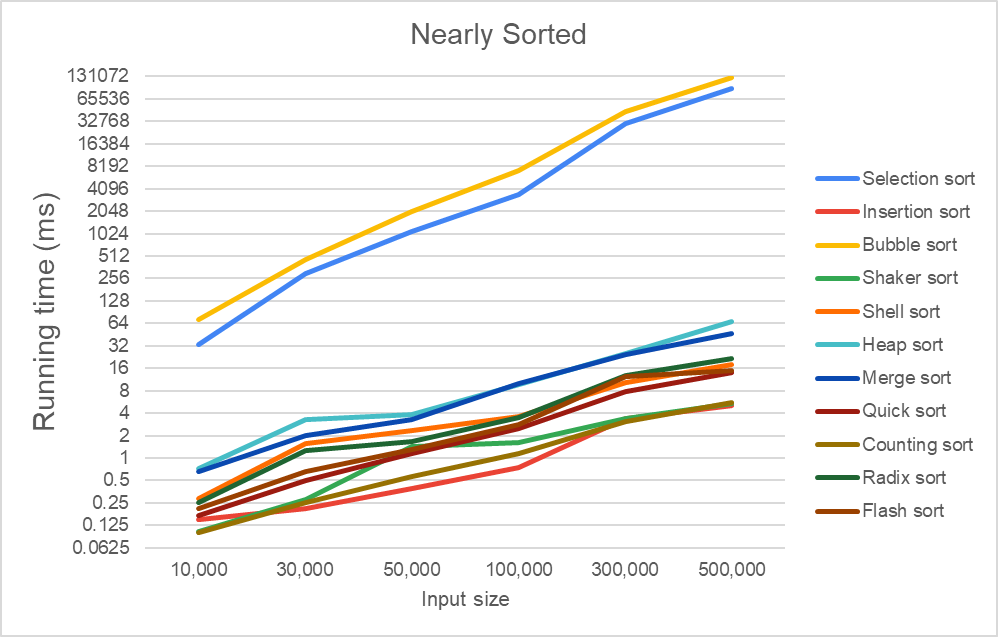
\includegraphics[width = 0.9\linewidth]{img/experiment/running time/nearly sorted/1.png}
    \caption{Thời gian chạy của các thuật toán trên bộ dữ liệu gần như được sắp xếp}
\end{figure}

\begin{figure}[H]
    \centering
    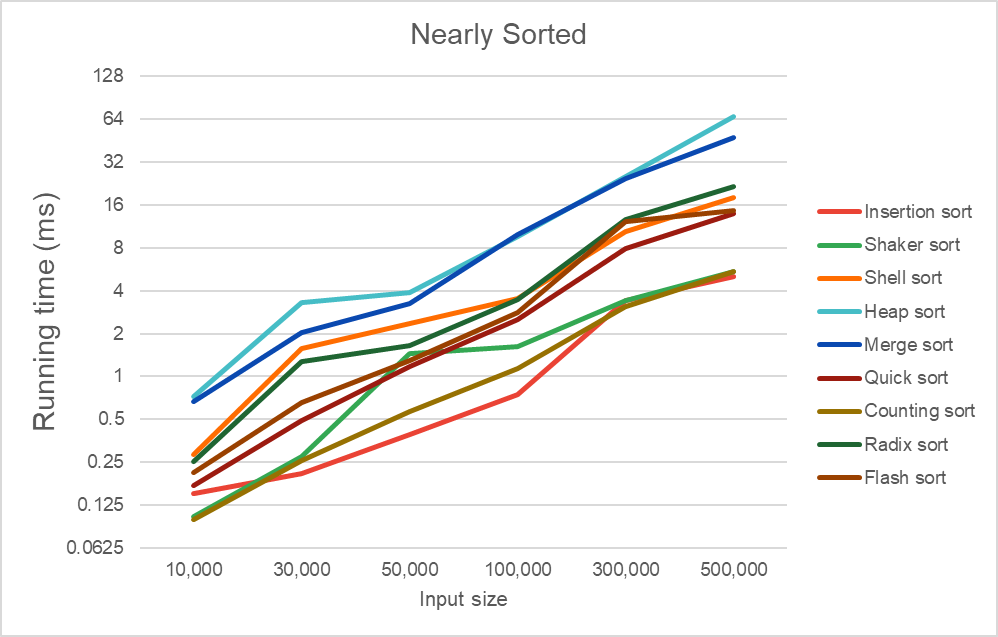
\includegraphics[width = 0.9\linewidth]{img/experiment/running time/nearly sorted/2.png}
    \caption{Thời gian chạy của các thuật toán chạy nhanh trên bộ dữ liệu gần như được sắp xếp}
\end{figure}

\begin{figure}[H]
    \centering
    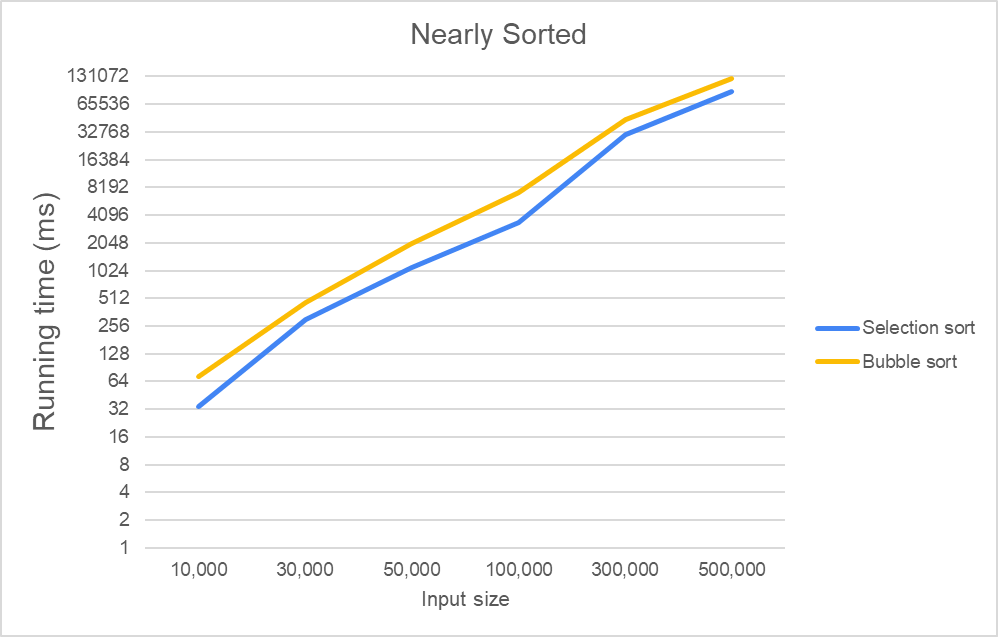
\includegraphics[width = 0.9\linewidth]{img/experiment/running time/nearly sorted/3.png}
    \caption{Thời gian chạy của các thuật toán chạy chậm trên bộ dữ liệu gần như được sắp xếp}
\end{figure}

\begin{itemize}
    \item \textbf{Hiệu năng tốt nhất:} Insertion sort.
    \item \textbf{Hiệu năng tệ nhất:} Bubble sort.
    \item Bộ dữ liệu gần như đã được sắp xếp nên có 1 số thuật toán có thể nhận diện được điều này và giảm được thời gian chạy, nhưng lúc này lại có một số thuật toán có thời gian chạy thiếu sự ổn định.
    \item \textit{Selection sort, Bubble sort:} Tương tự với trường hợp dữ liệu được sắp xếp, cả 2 thuật toán này đều có thời gian chạy tăng nhanh theo kích thước của bộ dữ liệu.
    \item \textit{Insertion sort, Shaker sort:} Tuy vẫn có hiệu năng tốt tương tự với bộ dữ liệu được sắp xếp nhưng lúc này thời gian chạy của cả 2 lại thiếu ổn định. \textit{Insertion sort} lại có hiệu năng tốt hơn \textit{Shaker sort} vì \textit{Insertion sort} đưa các phần tử về đúng vị trí của nó trong mảng cần được sắp xếp với rất ít các phép so sánh và hoán đổi, còn \textit{Shaker sort} lại cần vài lần duyệt mảng. Do đó \textit{Insertion sort} trở thành lựa chọn tốt nhất trong trường hợp dữ liệu gần như được sắp xếp.
    \item \textit{Shell sort:} Tương tự với trường hợp dữ liệu được sắp xếp, \textit{Shell sort} có thời gian chạy tốt và cũng khá ổn định.
    \item \textit{Heap sort, Merge sort, Quick sort:} Tương tự với trường hợp dữ liệu được sắp xếp, các thuật toán đều có thời gian chạy ổn định và tăng chậm.
    \item \textit{Counting sort, Radix sort, Flash sort:} Tương tự với trường hợp dữ liệu được sắp xếp, các thuật toán đều có thời gian chạy ổn định và tăng chậm.
\end{itemize}

\newpage
\begin{figure}[H]
    \centering    
    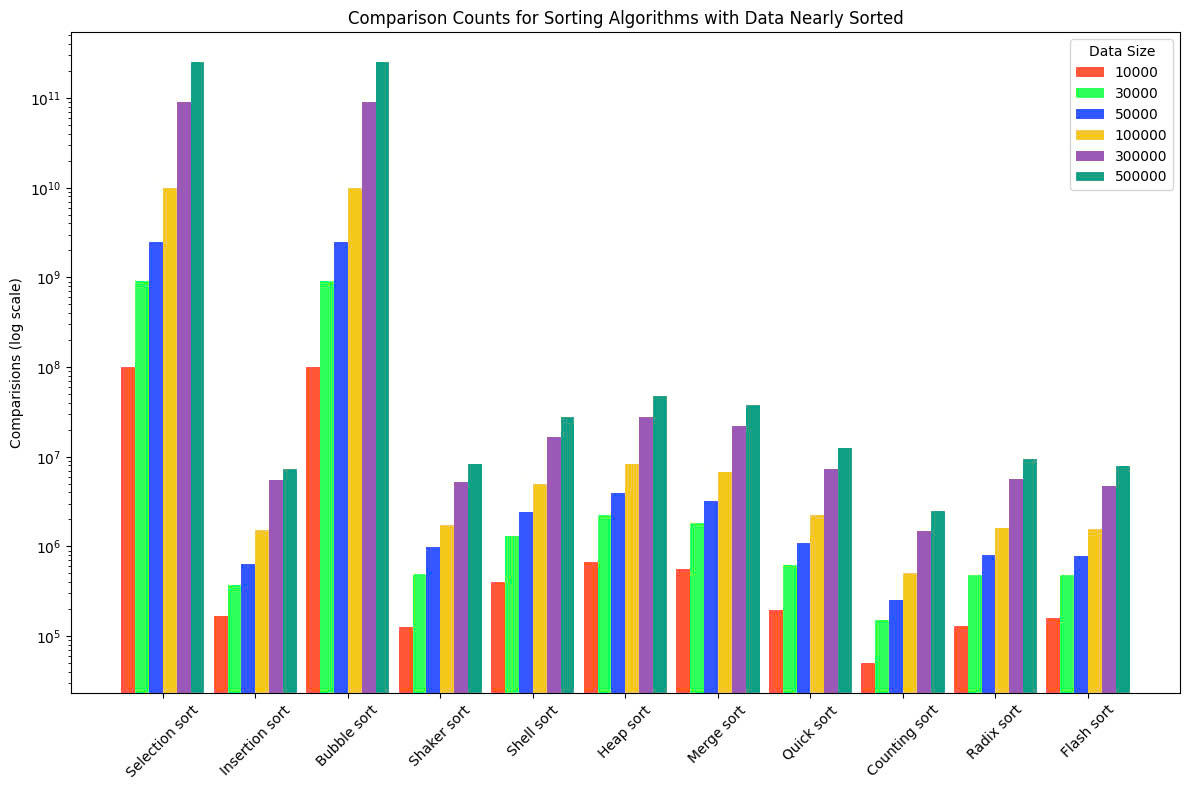
\includegraphics[width = 1\linewidth]{img/experiment/comparison/COMPARISON_NEARLY.jpg}
    \caption{Biểu đồ số lượng phép so sánh của các thuật toán trên bộ dữ liệu gần như được sắp xếp}
\end{figure}
\paragraph{Quan sát biểu đồ cột:}
\begin{itemize}
    \item \textbf{Số phép so sánh ít nhất:} Insertion sort.
    \item \textbf{Số phép so sánh nhiều nhất:} Selection sort.
    \item \textit{Selection sort, Bubble sort:} Các thuật toán này đều có số phép so sánh nhiều nhất và số phép tang nhanh khi kích thước mảng tăng lên. \textit{Selection sort} là thuật toán có nhiều phép so sánh nhất trong nhóm này vì luôn phải thực hiện $\frac{n(n-1)}{2}$ phép so sánh mà không phụ thuộc vào tính chất bộ dữ liệu.
    \item \textit{Insertion sort, Shaker sort: }Khi dữ liệu gần như đã được sắp xếp, \textit{Insertion sort} và \textit{Shaker sort} thể hiện rõ ưu thế vượt trội, với số phép so sánh giảm đáng kể so với các thuật toán khác. Đây là lựa chọn lý tưởng trong trường hợp dữ liệu gần như được sắp xếp.
    \item \textit{Quick sort: }Số phép so sánh tương đối thấp trong trường hợp này, nhưng không tối ưu bằng \textit{Insertion sort} và \textit{Shaker sort} khi dữ liệu gần như sắp xếp.
    \item \textit{Shell sort, Merge sort, Heap sort: }Các thuật toán này duy trì số phép so sánh ổn định hơn và không bị ảnh hưởng lớn bởi dữ liệu gần như sắp xếp.
    \item \textit{Counting sort, Radix sort, Flash sort:} Các thuật toán này sắp xếp đều không phụ thuộc vào việc so sánh giữa giá trị của các phần tử nên có số phép so sánh ít và không tăng nhanh khi kích thước mảng tăng lên vì nó không dựa vào việc so sánh phần tử.
\end{itemize}
%---------------------------------------------------------------------------------------------------------------
% Reversed data
\newpage
\subsubsection{Reversed data}
\begin{table}[!h]
    \centering
    \caption{Sorting Algorithms Performance (Data size: 10,000 to 50,000)}
    \resizebox{\textwidth}{!}{
    \begin{tabular}{|c|c|c|c|c|c|c|}
    \hline
    \multicolumn{7}{|c|}{Data order: Reversed} \\ \hline
    \textbf{Data size}         & \multicolumn{2}{c|}{10,000} & \multicolumn{2}{c|}{30,000} & \multicolumn{2}{c|}{50,000} \\ \hline
    \textbf{Resulting statics} & Running time    & Comparisons & Running time & Comparisons & Running time   & Comparisons   \\ \hline
    Selection sort             & $64.944162$     & $100009999$ & $482.474513$ & $900029999$ & $1462.290394$  & $2500049999$  \\ \hline
    Insertion sort             & $38.776609$     & $100009999$ & $291.697824$ & $900029999$ & $1605.098435$  & $2500049999$  \\ \hline
    Bubble sort                & $33.607111$     & $100009999$ & $334.683171$ & $900029999$ & $890.711355$   & $2500049999$  \\ \hline
    Shaker sort                & $44.056373$     & $100005001$ & $436.530637$ & $900015001$ & $1294.37119$   & $2500025001$  \\ \hline
    Shell sort                 & $0.31105$       & $475175$    & $0.950532$   & $1554051$   & $2.244672$     & $2844628$     \\ \hline
    Heap sort                  & $0.770256$      & $606771$    & $2.346656$   & $2063324$   & $4.339417$     & $3612724$     \\ \hline
    Merge sort                 & $0.988753$      & $476441$    & $2.931055$   & $1573465$   & $4.25876$      & $2733945$     \\ \hline
    Quick sort                 & $0.18241$       & $203608$    & $0.501725$   & $657224$    & $1.286509$     & $1134456$     \\ \hline
    Counting sort              & $0.089557$      & $50002$     & $0.261799$   & $150002$    & $0.638524$     & $250002$      \\ \hline
    Radix sort                 & $0.306391$      & $160071$    & $0.929703$   & $480071$    & $1.71454$      & $800071$      \\ \hline
    Flash sort                 & $0.219089$      & $133252$    & $0.657466$   & $399752$    & $1.448604$     & $666252$      \\ \hline
    \end{tabular}}
    \end{table}

\begin{table}[!h]
    \centering
    \caption{Sorting Algorithms Performance (Data size: 100,000 to 500,000)}
    \resizebox{\textwidth}{!}{
    \begin{tabular}{|c|c|c|c|c|c|c|}
    \hline
    \multicolumn{7}{|c|}{Data order: Reversed} \\ \hline
    \textbf{Data size}         & \multicolumn{2}{c|}{100,000} & \multicolumn{2}{c|}{300,000} & \multicolumn{2}{c|}{500,000}   \\ \hline
    \textbf{Resulting statics} & Running time    & Comparisons   & Running time   & Comparisons   & Running time  & Comparisons     \\ \hline
    Selection sort             & $6120.243176$   & $10000099999$ & $46520.55081$  & $90000299999$ & $91411.25704$ & $250000499999$  \\ \hline
    Insertion sort             & $5126.443574$   & $10000099999$ & $30450.51308$  & $90000299999$ & $104870.0817$ & $250000499999$  \\ \hline
    Bubble sort                & $3452.410914$   & $10000099999$ & $31193.35321$  & $90000299999$ & $86570.30637$ & $250000499999$  \\ \hline
    Shaker sort                & $4536.157937$   & $10000050001$ & $41117.02668$  & $90000150001$ & $114949.2044$ & $250000250001$  \\ \hline
    Shell sort                 & $4.157031$      & $6089190$     & $11.658126$    & $20001852$    & $19.676737$   & $33857581$      \\ \hline
    Heap sort                  & $9.219246$      & $7718943$     & $27.390857$    & $25569379$    & $59.587822$   & $44483348$      \\ \hline
    Merge sort                 & $11.226081$     & $5767897$     & $23.998696$    & $18708313$    & $58.800378$   & $32336409$      \\ \hline
    Quick sort                 & $2.824666$      & $2368920$     & $8.391546$     & $7575704$     & $9.597054$    & $12975704$      \\ \hline
    Counting sort              & $0.914415$      & $500002$      & $2.761508$     & $1500002$     & $4.665379$    & $2500002$       \\ \hline
    Radix sort                 & $4.246591$      & $1900085$     & $11.667985$    & $5700085$     & $19.34052$    & $9500085$       \\ \hline
    Flash sort                 & $2.194011$      & $1332502$     & $6.825843$     & $3997502$     & $11.320678$   & $6662502$       \\ \hline
    \end{tabular}}
\end{table}
    \begin{figure}[H] 
        \centering
        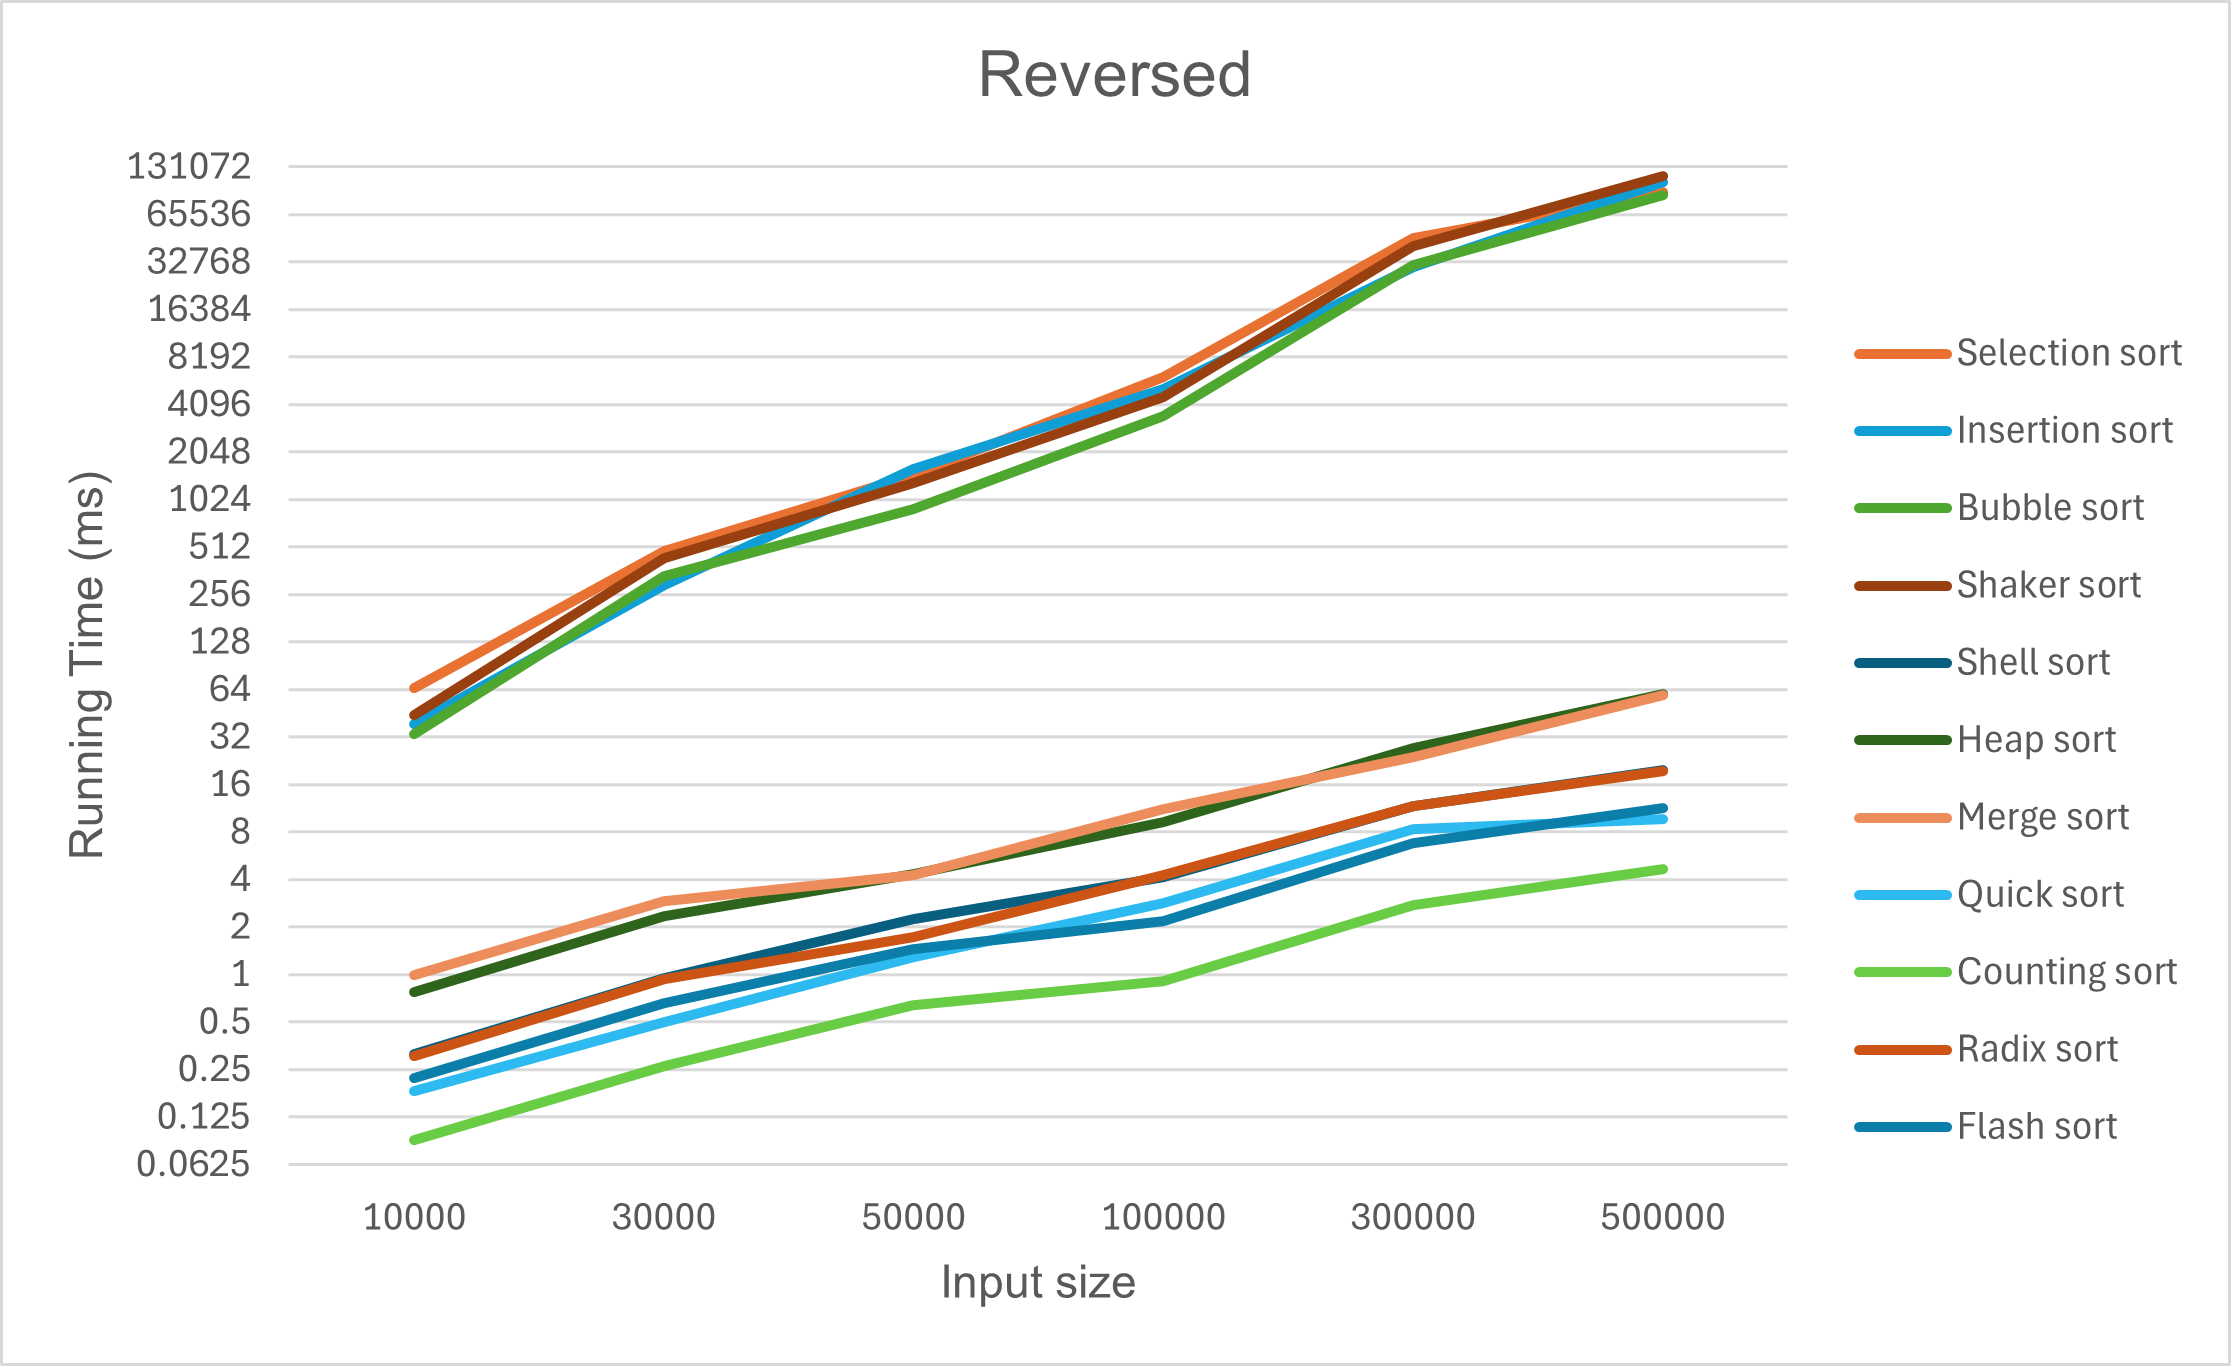
\includegraphics[width = 0.9\linewidth]{img/experiment/running time/reversed/1.png}
        \caption{Biều đồ thời gian chạy của các thuật toán trên bộ dữ liệu sắp xếp ngược}
    \end{figure}

    \begin{figure}[H]
        \centering
        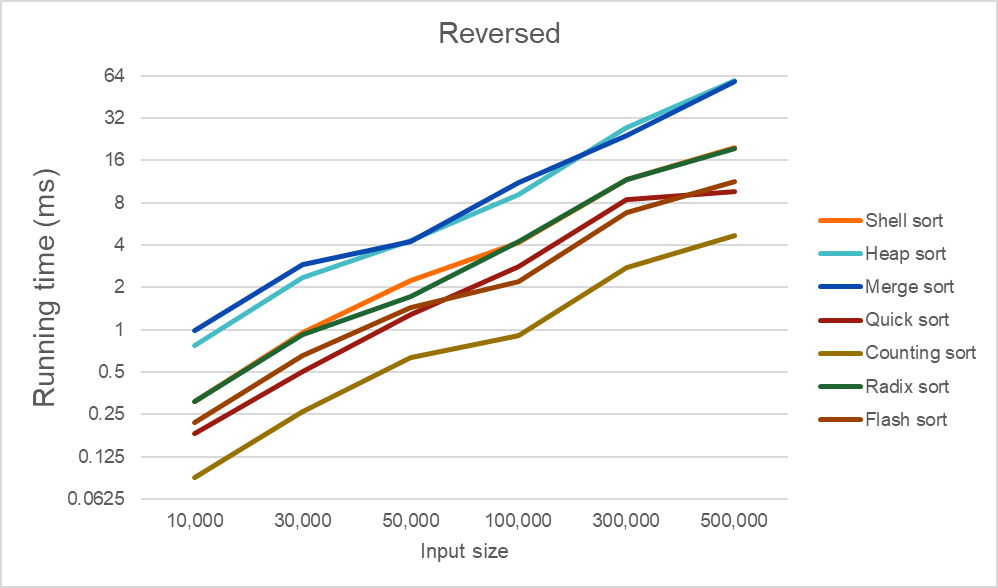
\includegraphics[width = 0.9\linewidth]{img/experiment/running time/reversed/2.png}
        \caption{Biểu đồ thời gian chạy của nhóm thuật toán có thời gian chạy nhanh trên bộ dữ liệu sắp xếp ngược}
    \end{figure}

    \begin{figure}[H]
        \centering
        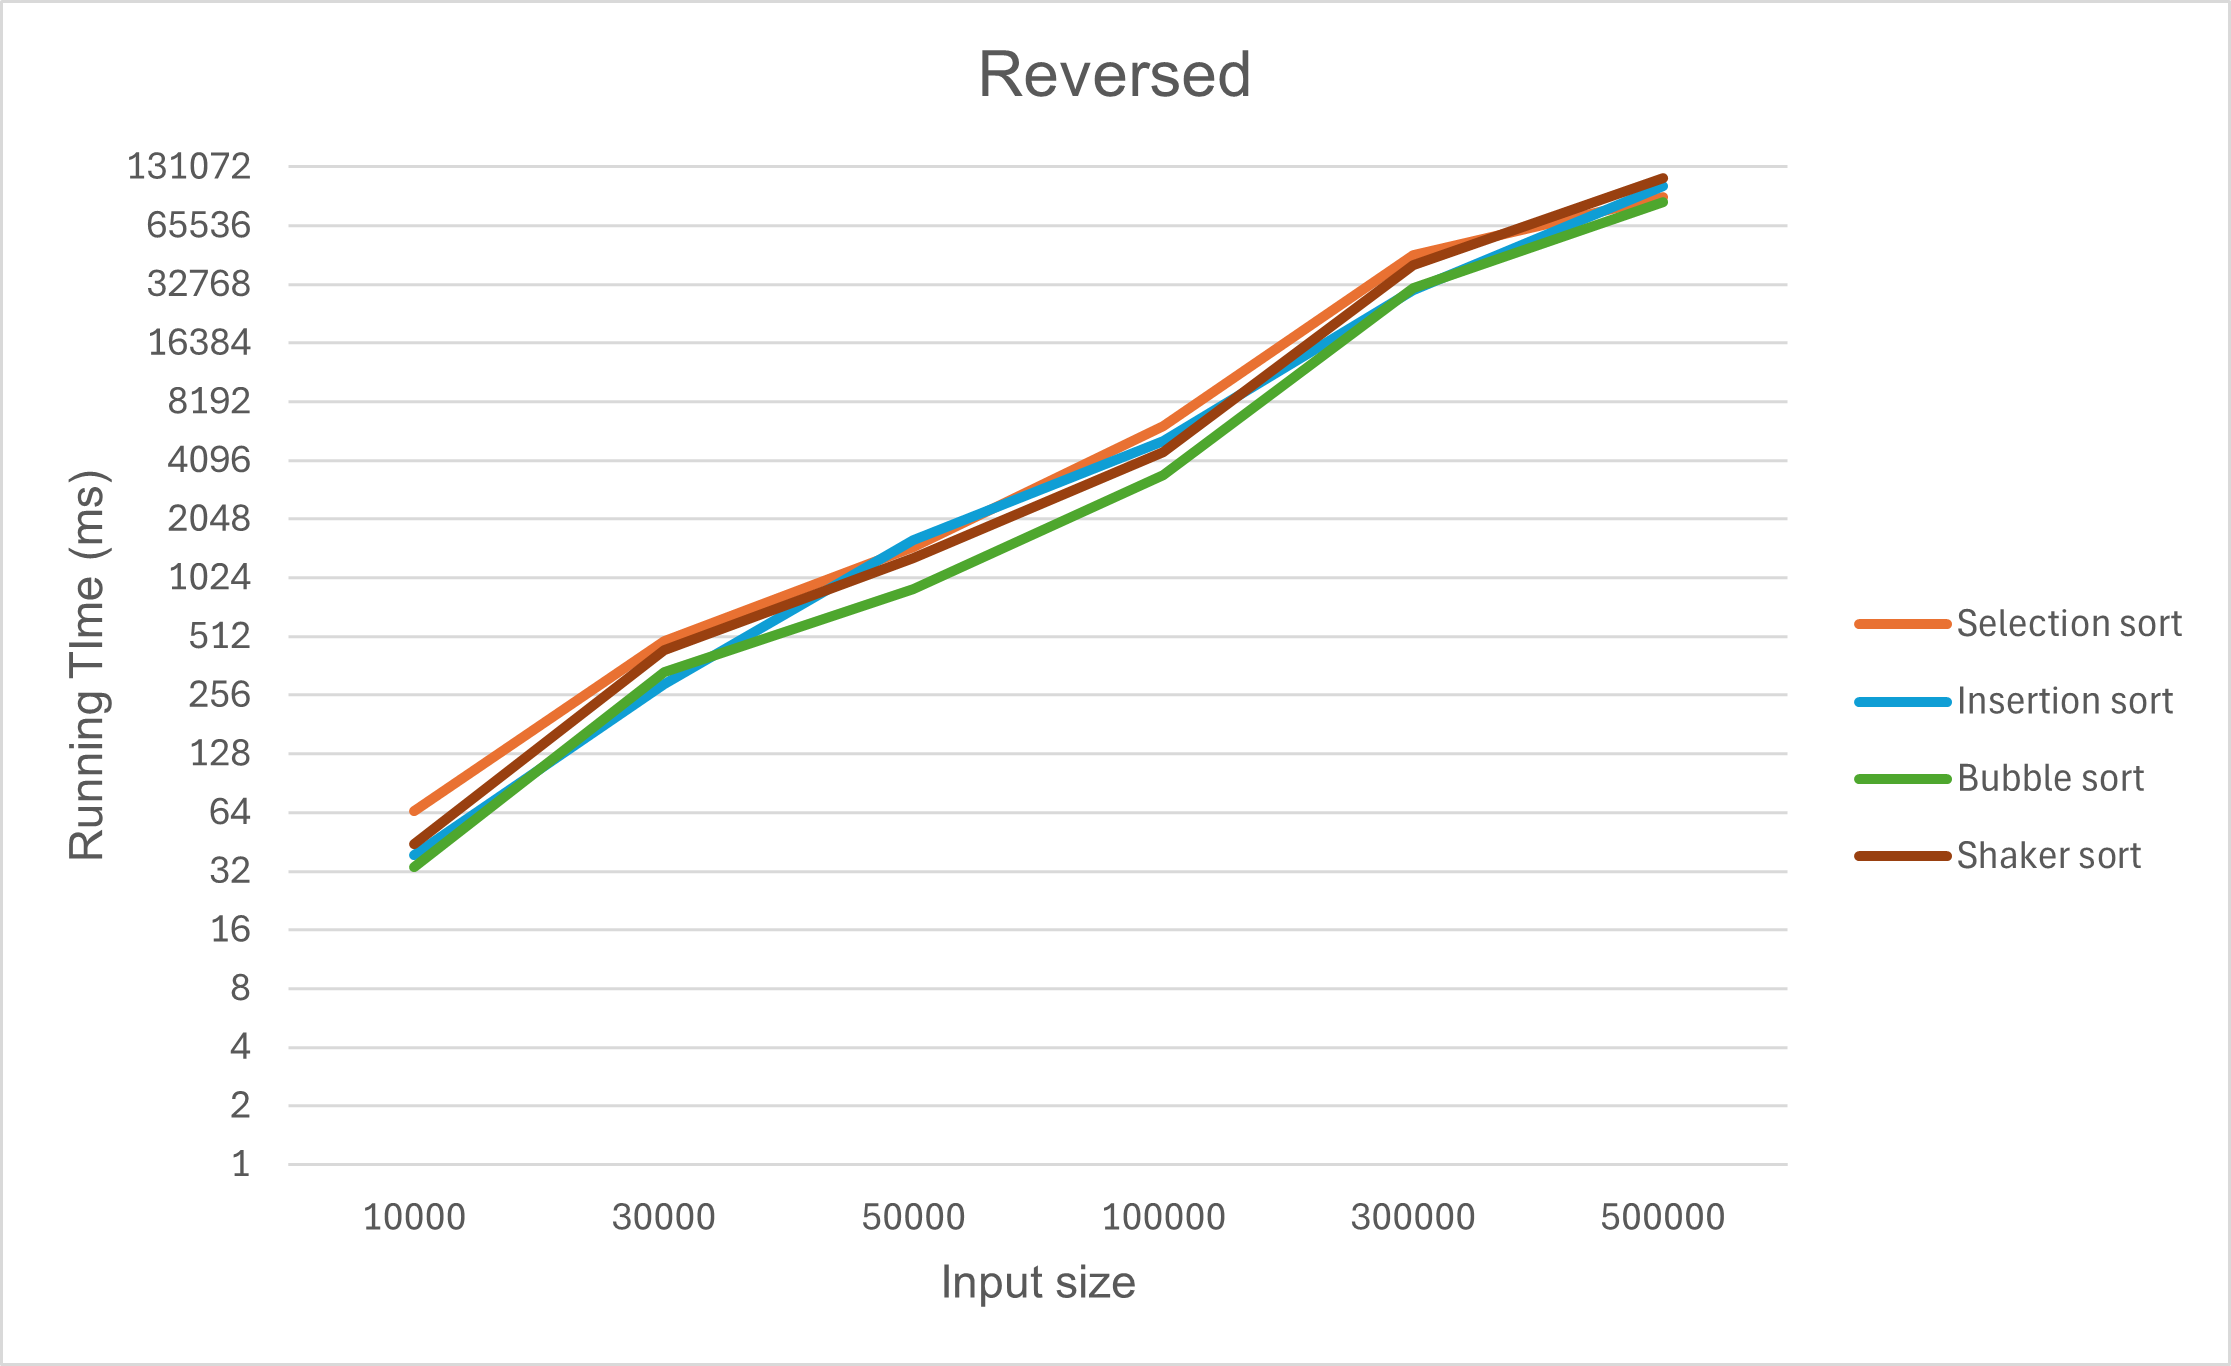
\includegraphics[width = 0.9\linewidth]{img/experiment/running time/reversed/3.png}
        \caption{Biểu đồ thời gian chạy của nhóm thuật toán có thời gian chạy chậm trên bộ dữ liệu sắp xếp ngược}
    \end{figure}

    \paragraph{Quan sát biểu đồ đường:}
    \begin{itemize}
        \item \textbf{Hiệu năng tốt nhất:} Counting sort.
        \item \textbf{Hiệu năng tệ nhất:} Selection sort. 
        \item \textit{Selection sort, Bubble sort, Insertion sort, Shaker sort:} Các thuật toán này đều có thời gian chạy tăng nhanh theo kích thước của bộ dữ liệu, điều này phù hợp với độ phức tạp lý thuyết $\mathcal{O}(n^2)$, yêu cầu số lượng phép so sánh rất lớn để đưa các phần tử về đúng vị trí dẫn đến thời gian chạy chậm.
        \item \textit{Shell sort, Heap sort, Merge sort, Quick sort:} Các thuật toán này đều có thời gian chạy ổn định và tăng chậm, phù hợp với độ phức tạp $\mathcal{O}(n \cdot \log n)$. Trong nhóm này \textit{Quick sort} vẫn có hiệu năng tốt nhất do sử dụng pivot ở giữa mảng, cách chọn này giúp tránh được các tình huống xấu nhất đặc biệt trong mảng có phân phối dữ liệu đều, điều này còn giúp giảm nguy cơ phân chia không cân đối trong gọi đệ quy.
        \item \textit{Counting sort, Radix sort, Flash sort:} Các thuật toán này khộng phụ thuộc vào sắp xếp dữ liệu mà thuộc vào phân phối dữ liệu đối với \textit{Flash sort}, phạm vi giá trị của mảng đối với \textit{Radix sort} và \textit{Counting sort} nên với bộ dữ liệu ngược thì các thuật toán này vẫn giữ được hiệu năng tốt.
    \end{itemize}

    \newpage

    \begin{figure}[H]
        \centering
        \includegraphics[width = 0.9\linewidth]{img/experiment/comparison/reversed.png}
        \caption{Biểu đồ số lượng phép so sánh của các thuật toán trên bộ dữ liệu sắp xếp ngược}
    \end{figure}

    \paragraph{Quan sát biểu đồ cột:}
    \begin{itemize}
        \item \textbf{Số phép so sánh ít nhất:} Counting sort.
        \item \textbf{Số phép so sánh nhiều nhất:} Selection sort.
        \item \textit{Selection sort, Bubble sort, Insert sort, Shaker sort:} Các thuật toán này đều có số phép so sánh nhiều nhất và số phép tang nhanh khi kích thước mảnh tăng lên. \textit{Selection sort} là thuật toán có nhiều phép so sánh nhất trong nhóm này vì luôn phải thực hiện $\frac{n(n-1)}{2}$ phép so sánh dù bộ dữ liệu đã được sắp xếp ra sao.
        \item \textit{Shell sort, Heap sort, Merge sort, Quick sort:} Các thuật toán này đều có số phép so sánh ít nhất và tăng chậm khi kích thước mảng tăng lên. \textit{Quick sort} vẫn là thuật toán có hiệu năng tốt nhất trong nhóm này.
        \item \textit{Counting sort, Radix sort, Flash sort:} Các thuật toán này sắp xếp đều không phụ thuộc vào việc so sánh giữa giá trị của các phần tử nên có số phép so sánh ít nhất và không tăng nhanh khi kích thước mảng tăng lên.
    \end{itemize}



\newpage
\subsection{Kết luận}

\textbf{Nhóm thuật toán có tốc độ nhanh nhất:}

\begin{itemize}
    \item \textbf{Đối với bộ dữ liệu ngẫu nhiên (Randomize):} Counting Sort, Radix Sort, và Flash Sort là những thuật toán có tốc độ nhanh nhất. Tốc độ chạy của cả ba thuật toán này không phụ thuộc vào thứ tự sắp xếp của mảng, mà chủ yếu dựa vào đặc tính của dữ liệu. Cụ thể: Counting Sort và Radix Sort phụ thuộc vào khoảng giá trị của các phần tử, trong khi Flash Sort phụ thuộc vào sự phân bố giá trị trong mảng.
    
    \item \textbf{Đối với bộ dữ liệu đã sắp xếp (Sorted) và gần sắp xếp (Nearly Sorted):} Shaker Sort và Insertion Sort là hai thuật toán vượt trội nhất. Cả hai thuật toán chỉ thực hiện một lượt kiểm tra các phần tử, đạt độ phức tạp $\mathcal{O}(n)$. Trong khi đó, mặc dù Flash Sort cũng có độ phức tạp trung bình là $\mathcal{O}(n)$ trên các dữ liệu có phân phối đồng đều, thuật toán này vẫn chậm hơn do phải thực hiện thêm bước phân phối lại các giá trị, không tận dụng được đặc tính đã sắp xếp của mảng.
    
    \item \textbf{Đối với bộ dữ liệu sắp xếp ngược (Reversed):} Counting Sort là thuật toán có tốc độ nhanh nhất, nhờ vào cơ chế xử lý không phụ thuộc thứ tự ban đầu của mảng.
\end{itemize}

\textbf{Nhóm thuật toán có tốc độ chậm nhất:}

\begin{itemize}
    \item \textbf{Đối với tất cả các bộ dữ liệu:} Bubble Sort và Selection Sort là hai thuật toán chậm nhất. Nguyên nhân là cả hai không tận dụng được trạng thái của mảng (như đã sắp xếp hay gần sắp xếp). Bất kể dữ liệu đầu vào, chúng đều phải thực hiện toàn bộ các phép so sánh và hoán đổi (hoặc lựa chọn phần tử), dẫn đến độ phức tạp $\mathcal{O}(n^2)$ trong mọi trường hợp, làm giảm hiệu quả trên các bộ dữ liệu lớn.
\end{itemize}

\textbf{Tính ổn định của thuật toán}
\begin{itemize}
    \item \textbf{Thuật toán ổn định:} Counting Sort, Radix Sort, Bubble Sort, Insertion Sort, Merge Sort và Shaker Sort là các thuật toán ổn định. Điều này có nghĩa là thứ tự tương đối của các phần tử có giá trị bằng nhau trong mảng sẽ được duy trì sau khi sắp xếp.
    
    \item \textbf{Thuật toán không ổn định:} Flash Sort, Selection Sort, Quick Sort, Shell Sort, và Heap Sort không đảm bảo tính ổn định.
\end{itemize}
\newpage